\section{Blatt}


\begin{aufg}[6 Punkte]
Romeo m\"ochte Julia besuchen, aber zwischen den beiden ist ein $9$ Meter breiter Fluss. Romeo hat beliebig viele Holzbalken der L\"ange~$1$~m (Breite ~$50$ cm, H\"ohe $10$~cm) zur Verf\"ugung, aus denen er versucht will, eine Br\"ucke von der Form wie im Bild unten (Abbildung~\ref{fig:romeo}) zu bauen. Weiterhin hat er ein beliebig langes Seil, das er am oberen Ende der Br\"ucke befestigen will, um sich herunterzulassen. Die Br\"ucke ist stabil, wenn f\"ur jeden benutzten Holzbalken gilt, dass der Schwerpunkt der Brückenkonstruktion auf diesem Holzbalken \"uber diesem Holzbalken liegt. Das Gewicht von Romeo und dem Seil d\"urfen wir vernachl\"assigen, ebenso die m\"oglichen Probleme bei der Anbringung des Seiles. Schafft Romeo es, zu Julia zu kommen? (Genaue Begr\"undung!)
%
\begin{figure}
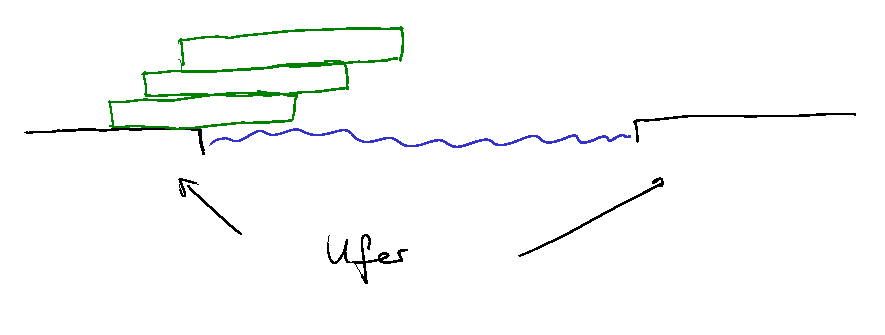
\includegraphics{romeo.pdf}
\caption{Romeos Br\"ucke}\label{fig:romeo} 
\end{figure}
%
\end{aufg}

\bigskip

\begin{lsg}
\end{lsg}


\bigskip


\begin{aufg}[6 Punkte]
Bestimmen Sie folgende Grenzwerte:
\begin{enumerate}[label=$\mathrm{(\roman*)}$, ref=$\mathrm{\roman*}$]
\setlength{\itemsep}{4pt}
\item $ \lim\limits_{x\to \infty} \dfrac{x^{2021}-17x^{10}}{x^{2022}+x+3} $,
\item $ \lim\limits_{x\to 2} \dfrac{x^{2}-3x+2}{x^{2}-x-2} $,
\item $ \lim\limits_{x\to 2} \left(1-\dfrac{2}{x}\right)^{2} \left( \dfrac{x^{7}-4x}{(x-2)^{2}} \right) $.
\end{enumerate}
\end{aufg}

\bigskip

\begin{lsg}[Arne Meyer, Simon Bruns]
\begin{enumerate}[label=$\mathrm{(\roman*)}$, ref=$\mathrm{\roman*}$]
\setlength{\itemsep}{4pt}
\item\[\lim_{x \to\infty}\frac{x^{2021}-17x^{10}}{x^{2022}+x+3} =\lim_{x \to\infty} \frac{\frac{1}{x}-\frac{17}{x^{2012}}}{1+\frac{1}{x^{2021}}+\frac{3}{x^{2022}}}=0 \]		
\item\[\lim_{x \to 2}\frac{x^{2}-3x+2}{x^{2}-x-2}= \lim_{x \to 2} \frac{(x-2)(x-1)}{(x-2)(x+1)}=\frac{1}{3}\]
\item\[ \lim_{x \to 2}\left(1-\frac{2}{x}\right)^2\left(\frac{x^7-4x}{\left(x-2\right)^2}\right)=\lim_{x \to 2}\left(\frac{x-2}{x}\right)^2    \cdot \frac{x^7-4x}{(x-2)^2}=\lim_{x \to 2} \frac{x^6-4}{x}= 30\] 
\end{enumerate}
\end{lsg}

\bigskip 


\begin{lsg}[Yan Lin, Yunling Yang]\mbox{ }
\begin{enumerate}[label=$\mathrm{(\roman*)}$, ref=$\mathrm{\roman*}$]
\item Die Funktionen auf dem Z\"ahler und Nenner sind Polynome. Deshalb sind 
die gesamte Funktion stetig, gleichfalls bei (ii) und (iii).
\begin{flalign}
& \lim_{x\to \infty} \frac{x^{2021}-17x^{10}}{x^{2022} + x +3} && \nonumber \\
 =& \lim_{x\to \infty} 
\frac{1-\frac{17}{x^{2011}}}{x+\frac{1}{x^{2020}}+\frac{3}{x^{2021}}} && 
\nonumber \\
 =& \lim_{x\to \infty} \frac{1}{x} && \nonumber \\
 =& \: 0 \nonumber
\end{flalign}
%
\item 
\begin{flalign}
 &\lim_{x \to 2} \frac{x^2-3x+2}{x^2-x-2} && \nonumber\\
=& \lim_{x \to 2} \frac{(x-2)(x-1)}{(x-2)(x+1)}  \nonumber\\
=& \lim_{x \to 2} \frac{x-1}{x+1} \nonumber \\
=& \:\frac{1}{3} \nonumber
\end{flalign}
%
\item 
\begin{flalign}
& \lim_{x \to 2} \left( 1 - 
\frac{2}{x}\right)^2\left(\frac{x^7-4x}{(x-2^2)}\right) && \nonumber \\
=& \lim_{x \to 2} \left(\frac{1-\frac{2}{x}}{x-2}\right)^2 \cdot (x^7-4x) && 
\nonumber \\
=& \lim_{x \to 2} \frac{x^7-4x}{x^2} && \nonumber \\
=& \lim_{x \to 2} x^5-\frac{4}{x} && \nonumber \\
=& \: 30 \nonumber
\end{flalign}
\end{enumerate}
\end{lsg}


\bigskip

\begin{aufg}[6 Punkte]
Die Exponentialfunktion $\exp\colon\R\to\R$ ist gegeben durch (siehe Vorlesung)
\[
\exp(x)\coloneqq \sum_{k=0}^{\infty}\frac{x^k}{k!}\,. 
\]
\begin{enumerate}[label=$\mathrm{(\roman*)}$, ref=$\mathrm{\roman*}$]
\item Zeigen Sie, dass $\exp(x)\cdot \exp(y)=\exp(x+y)$ \emph{(Hinweis: Cauchy-Produkt)}.
\item Zeigen Sie, dass die Exponentialfunktion auf ganz $\R$ stetig ist, d.h., f\"ur jedes~$x_0\in\R$ ist der Grenzwert von~$\exp$ in~$x_0$ gerade $\exp(x_0)$.
\end{enumerate}
\end{aufg}
 
\bigskip

\begin{lsg}\mbox{Lennart Koliwer, Tjado Edzards, Jonas Dierks, Robin Dornhoff}
\begin{enumerate}[label=$\mathrm{(\roman*)}$, ref=$\mathrm{\roman*}$]
\item
Z.z.:
\begin{align*}
\text{exp}(x) \cdot \text{exp}(y) = \text{exp}(x+y) &\Leftrightarrow \sum_{k=0}^{\infty}\frac{x^k}{k!}\cdot \sum_{k=0}^{\infty}\frac{y^k}{k!} = \sum_{k=0}^{\infty}\frac{(x+y)^k}{k!}
\\
\intertext{Mit dem Cauchy-Produkt ergibt sich aus exp($x$)exp($y$) folgendes:}
\sum_{k=0}^{\infty}\frac{x^k}{k!}\cdot \sum_{k=0}^{\infty}\frac{y^k}{k!} &= \sum_{k=0}^{\infty}\sum_{n=0}^{k}\frac{x^n}{n!}\cdot \frac{y^{k-n}}{(k-n)!}
\\
\intertext{Zur Vereinfachung wird die Summe mit 1 multipliziert.}
&=\sum_{k=0}^{\infty}\sum_{n=0}^{k}\frac{x^n}{n!}\cdot \frac{y^{k-n}}{(k-n)!}\cdot \frac{k!}{k!}
\\
&=\sum_{k=0}^{\infty}\sum_{n=0}^{k}\frac{k!\cdot x^n\cdot y^{k-n}}{n!\cdot(k-n)!}\cdot \frac{1}{k!}
\intertext{Dabei lässt sich der Binomialkoeffizient finden.}
&=\sum_{k=0}^{\infty}\sum_{n=0}^{k}\binom{k}{n} \cdot x^n\cdot y^{k-n} \cdot \frac{1}{k!}
\\
&=\sum_{k=0}^{\infty}\frac{1}{k!}\sum_{n=0}^{k}\binom{k}{n} \cdot x^n\cdot y^{k-n}
\intertext{Cool das haben wir ja schon bewiesen :) Blatt 5 Binomischer Lehrsatz: $\sum_{n=0}^{k}\binom{k}{n} \cdot x^n\cdot y^{k-n} = (x+y)^k$}
&=\sum_{k=0}^{\infty}\frac{1}{k!}\cdot (x+y)^k
\\
\text{exp}(x+y)&=\sum_{k=0}^{\infty}\frac{(x+y)^k}{k!}
\end{align*}
\item Um zu beweisen, dass die Exponentialfunktion stetig ist, zeigen wir zunächst, dass die Exponentialfunktion an der Stelle $0$ stetig ist.
 
 Um also zu zeigen, dass
 \begin{align*}
  \forall \e >0: (\exists \D>0: (\forall x \in \textrm{U}_\D(0):|\textrm{exp}(x)-\textrm{exp}(0)|<\e))
 \end{align*} gilt, halten wir zunächst fest, dass
 \begin{align*}
  \textrm{exp}(0)= \sum_{k=0}^\infty \frac{0^k}{k!}=\frac{0^0}{0!}+ \sum_{k=1}^\infty 0 =1+0= 1
 \end{align*}ist.
 
 Nun sei $\e$ eine beliebige aber feste positive reele Zahl. Wir setzen $\D=1-\frac{1}{\e+1}\in \R$, sodass $0<\D<1$
 gilt.
 
 Nun zeigen wir, dass für alle $x\in \textrm{U}_\D(0)$, die größer als $0$ sind,
 $|\textrm{exp}(x)-\textrm{exp}(0)|<\e$ gilt.
 
 Dafür stellen wir zunächst fest, dass für solche $x$ gerade $\textrm{exp}(x)>1$ gilt, den mit der gegebenen Definition der Exponentialfunktion ergibt sich rechnerisch mit weiterhin $x>0$ gerade
 \begin{align*}
  \textrm{exp}(x)= \sum_{k=0}^\infty \frac{x^k}{k!}= \sum_{k=0}^0 \frac{x^k}{k!}+ \sum_{k=1}^\infty \frac{x^k}{k!}= \frac{x^0}{0!}+\sum_{k=1}^\infty \frac{x^k}{k!}= 1+\underbrace{\sum_{k=1}^\infty \frac{x^k}{k!}}_{\textrm{stets positiv, da stets}\; x>0 \; \textrm{und}\; k>0 }>1,
 \end{align*} sodass für diese $x$ gerade
 \begin{align*}
  \textrm{exp}(x)-1>0
 \end{align*}
 und folglich\begin{align*}
  |\textrm{exp}(x)-\textrm{exp}(0)|= |\textrm{exp}(x)-1|<\e \Leftrightarrow \textrm{exp}(x)-1<\e
 \end{align*} gilt, sodass für uns der Beweis der letzteren Aussage ausreicht.
 
Für den Beweis der besagten Aussage nutzen wir aus, dass da weiterhin die betrachteten $x>0$ in der $\D-$Umgebung von $0$ sind,also  mit den bisherigen Ausführungen
\begin{align*}
 0<x<\D<1
\end{align*} gilt, sodass wir mit dem Wissen über das Konvergenzverhalten der geometrischen Reihe gerade rechnerisch als wahre Aussage
\begin{align*}
  &\textrm{exp}(x)-1= \left(\sum_{k=0}^\infty \frac{x^k}{k!} \right)-1 \stackrel{\textrm{da} \; k \geq0}{<} \left(\sum_{k=0}^\infty x^k \right)-1 \stackrel{\textrm{da} \; 0< x< 1}{=} \frac{1}{1-x}-1\\ &\stackrel{\textrm{da} \; 0< x< \D< 1}{<} \frac{1}{1-\D} -1\stackrel{\textrm{nach Wahl von} \; \D}{=} \frac{1}{1-\left(1-\frac{1}{\e+1}\right)}-1 = \e
 \end{align*}
erhalten, also mit der oben erwähnten Äquivalenz für alle $x>0$ in der $\D-$Umgebung von $0$ gerade
\begin{align*}
  |\textrm{exp}(x)-\textrm{exp}(0)|<\e
 \end{align*}
gilt.

Dass für $x=0$ in der $\D-$Umgebung von $0$ gerade
\begin{align*}
  |\textrm{exp}(x)-\textrm{exp}(0)|<\e
 \end{align*}
gilt, ist trivial, sodass wir nun noch für diesen Teil des Beweises der Stetigkeit der Exponentialfunktion nur noch zeigen müssen, dass für alle $x<0$ die in der $\D-$Umgebung von $0$ sind gerade
\begin{align*}
  |\textrm{exp}(x)-\textrm{exp}(0)|<\e
 \end{align*}
gilt.

Dafür können wir zunächst festhalten, dass das jeweils additiv Inverse $-x$ solcher $x$ offentsichtlich auch in der $\D-$Umgebung von $0$ ist, und dabei größer als $0$ ist, sodass mit den bisherigen Ausführungen für alle $x<0$ die in der $\D-$Umgebung von $0$ sind gerade
\begin{align*}
  |\textrm{exp}(-x)-\textrm{exp}(0)|<\e
 \end{align*}
und
\begin{align*}
  \textrm{exp}(-x)>1
 \end{align*}
 gilt.
 
 Nun nutzen wir Lemma (i) aus, nach dem mit $\textrm{exp}(0)=1$ gerade
 \begin{align*}
  \textrm{exp}(x) \cdot \textrm{exp}(-x)=\textrm{exp}(x+(-x))=\textrm{exp}(0)=1 \stackrel{\textrm{da} \; \textrm{exp}(-x) >1}{\Leftrightarrow} \textrm{exp}(x)= \frac{1}{\textrm{exp}(-x)}
 \end{align*}gilt, sodass wir für den Beweis, dass für die $x<0$ die in der $\D-$Umgebung von $0$ sind gerade
\begin{align*}
  |\textrm{exp}(x)-\textrm{exp}(0)|<\e
 \end{align*}
gilt, $\textrm{exp}(x)$ durch $\frac{1}{\textrm{exp}(-x)}$ substituieren können, sodass wir für die $x<0$ die in der $\D-$Umgebung von $0$ sind rechnerisch mit \newline $\textrm{exp}(-x)>1 \Leftrightarrow 0<\frac{1}{\textrm{exp}(-x)} <1 $ und $|\textrm{exp}(-x)-\textrm{exp}(0)|=|\textrm{exp}(-x)-1|<\e$ gerade
\begin{align*}
  &|\textrm{exp}(x)-\textrm{exp}(0)|= \left|\frac{1}{\textrm{exp}(-x)}-1\right| = \left|\frac{1-\textrm{exp}(-x)}{\textrm{exp}(-x)} \right|\\&= \left|\frac{1}{\textrm{exp}(-x)} \right|\cdot\left|1-\textrm{exp}(-x) \right|= \left|\frac{1}{\textrm{exp}(-x)} \right|\cdot\left|\textrm{exp}(-x)-1 \right|<\e
 \end{align*}
erhalten.

Somit gilt für ein beliebiges aber festes positives reeles $\e$, und somit für alle reele $\e>0$, dass mit $\D=1-\frac{1}{\e+1}$ ein $\D$ existiert, mit dem für alle $x$ in der $\D-$ Umgebung von $0$ gerade
\begin{align*}
  |\textrm{exp}(x)-\textrm{exp}(0)|<\e
 \end{align*}
gilt, sodass bewiesenermaßen die Exponentialfunktion an der Stelle $0$ stetig ist.
 
Nun beweisen wir noch, dass die Exponentialfunktion an einer beliebigen aber festen Stelle $\chi \in \R$ stetig ist, und somit die Exponentialfunktion stetig ist.

Dafür benutzen wir das Folgenkriterium, nach dem wir einerseits wissen, dass mit den bisherigen Resultaten für alle Folgen $(g_n)$ in $\R \setminus \{0\}$ mit $g_n \stackrel{n\to \infty}{\to}0$  gerade $\textrm{exp}(g_n) \stackrel{n\to \infty}{\to}\textrm{exp}(0)=1$ gilt, und andererseits die Exponentialfunktion an der Stelle $\chi$ genau dann stetig ist, wenn für eine beliebige aber feste Folge $(h_n)$ in $\R\setminus \{\chi\}$, die gegen $\chi$ konvergiert, gerade  $\textrm{exp}(h_n) \stackrel{n\to \infty}{\to}\textrm{exp}(\chi)$ gilt.

Sei also $(h_n)$ eine Folge, die gegen $\chi$ konvergiert, so wissen wir, dass die Folge $(i_n)$, mit $i_n=h_n-chi$, eine Nullfolge ist, sodass mit den bisherigen Ausführungen gerade
\begin{align*}
 \textrm{exp}(i_n)= \textrm{exp}(h_n-\chi) \stackrel{n\to \infty}{\to}\textrm{exp}(0)=1
\end{align*} gilt.

Hierraus folgt nach Lemma (i) und der obigen Überlegung, dass $\textrm{exp}(x)= \frac{1}{\textrm{exp}(-x)}$ mit $x \in \R$ gilt, dass mit $\chi$ einer beliebigen aber festen reelen Zahl und $(h_n)$ einer beliebigen aber festen Folge $(h_n)$ in $\R\setminus \{\chi\}$, die gegen $\chi$ konvergiert,
\begin{align*}
&\textrm{exp}(h_n-\chi)= \textrm{exp}(h_n) \cdot \textrm{exp}(-\chi)= \frac{\textrm{exp}(h_n)}{\textrm{exp}(\chi)}  \stackrel{n\to \infty}{\to}1\\ \Leftrightarrow &\textrm{exp}(h_n) \stackrel{n\to \infty}{\to}\textrm{exp}(\chi)
\end{align*} gilt.
 
Somit ist die Exponentialfunktion nach dem Folgenkriterium an der beliebigen aber festen reelen Stelle $\chi$ stetig, sodass die Exponentialfunktion stetig ist, quad erat demonstrandum.

\end{enumerate}
\end{lsg}

\bigskip


\begin{aufg}[6 Punkte]
Die \textit{Riemannsche Zeta-Funktion} wird definiert durch die Reihe 
\[
\zeta(s) = \sum_{k=1}^{\infty} \frac{1}{k^{s}}
\]
f\"ur alle $s\in \R$, $s>1$. Zeigen Sie, dass $\zeta(n) < 2$ f\"ur alle nat\"urlichen Zahlen $n\geq 2$. 

\noindent
\emph{Hinweis:} Betrachten Sie zuerst
\[
\sum_{n=2}^{\infty} \sum_{k=2}^{\infty} \frac{1}{k^{n}}\,.
\]
\end{aufg}


\bigskip

\begin{lsg}[Zehra Ciftci, Sude Cinar, Saveen Kassem]

Z.z.: $\zeta(n) < 2$ f\"ur alle nat\"urlichen Zahlen $n\geq 2$. 


Es gilt nach Beispiel 3.60: 

\[ \displaystyle\sum_{k=1}^{\infty}\frac{1}{k^{2}}\]

ist eine konvergente Majorante für

\[ \displaystyle\sum_{k=1}^{\infty}\frac{1}{k^{m}}\] 

mit natürlichem $m > 2$. Außerdem gilt: $k^m > k^2$  genau dann, wenn  
$$\frac{1}{k^2} < \frac{1}{k^m}$$.

Auch gilt, dass die erste Patrialsumme mit dem Wert 1 gleich ist.

In Übungsblatt 8 wurde bewiesen, dass 

\[ \displaystyle\sum_{k=1}^{\infty}\frac{2}{(k+1)}=2\]

eine konvergente Majorante für 

\[ \displaystyle\sum_{k=1}^{\infty}\frac{1}{k^{2}}\]

und dass das erste Glied der Reihe gleich ist.

Somit entspricht: 


\begin{align*}
 \displaystyle\sum_{k=1}^{\infty}\frac{1}{k^{2}} < 
\displaystyle\sum_{k=1}^{\infty}\frac{2}{(k+1)}=2.
\end{align*}

Nach dem Axiom der Transitivität der Anorndnung gilt: 
\begin{align*}
\displaystyle\sum_{k=1}^{\infty}\frac{1}{k^{m}} 
& < \displaystyle\sum_{k=1}^{\infty}\frac{1}{k^{2}}
\\
& < \displaystyle\sum_{k=1}^{\infty}\frac{2}{(k+1)}=2
\end{align*}

Nun kann man mit der Definition der Riemannschen-Zeta-Funktion ausdrücken, dass 
mit einer weiterhin natürlichen Zahl größer 2 folgendes gilt:
\begin{align*}
 \zeta(m) = \displaystyle\sum_{k=1}^{\infty}\frac{1}{k^{m}}
& <
\zeta(2) = \displaystyle\sum_{k=1}^{\infty}\frac{1}{k^{2}}
\\ 
& <
\displaystyle\sum_{k=1}^{\infty}\frac{2}{(k+1)}=2
\end{align*}

also kurz: $$ \zeta(m) < \zeta(2) < 2 $$.

Somit wurde $\zeta(n) < 2$ f\"ur alle nat\"urlichen Zahlen $n\geq 2$ gezeigt.
\end{lsg}
 
\bigskip

\begin{aufg}[2 Punkte; Sonderaufgabe]
Wenn Sie Aufgabe~8.5 abgegeben haben (womit Sie sich 2 Punkte verdient haben), erhalten Sie von ihrer \"Ubungsleiterin oder Ihrem \"Ubungsleiter die Abgabe einer anderen Gruppe. Korrigieren Sie diese Abgabe und bepunkten Sie sie. Sie haben 6 Punkte zur Verf\"ugung. (Die andere Gruppe erh\"alt nicht die Punkte, die Sie vergeben, sondern die 2 Punkte f\"ur das Abgeben.) Achten Sie beim Korrigieren insbesondere auf Folgendes: 
\begin{itemize}
 \item Alle Stellen, die falsch sind, anmerken und erkl\"aren, was falsch ist.
 \item Alle Stellen, die unverst\"andlich sind, anmerken und erkl\"aren, was unverst\"andlich ist.
\end{itemize}
Kurzum, Sie machen die Korrektur so, wie Sie erwarten, dass Ihre Abgaben korrigiert werden. Ihr Korrekturergebnis soll so sein, dass Sie hinterher erkl\"aren k\"onnen, was falsch und was richtig an der Abgabe ist. Sie geben die Korrektur dann mit Ihrer Abgabe von Blatt~9 am 21.12. in den \"Ubungsgruppen ab.
\end{aufg}

